\documentclass[a4paper,14pt]{article} % тип документа
%\documentclass[14pt]{extreport}
\usepackage{extsizes} % Возможность сделать 14-й шрифт


\usepackage{geometry} % Простой способ задавать поля
\geometry{top=20mm}
\geometry{bottom=25mm}
\geometry{left=15mm}
\geometry{right=15mm}

\setcounter{section}{0}

%%%Библиотеки
%\usepackage[warn]{mathtext}
%\usepackage[T2A]{fontenc} % кодировка
\usepackage[utf8]{inputenc} % кодировка исходного текста
\usepackage[english,russian]{babel} % локализация и переносы
\usepackage{caption}
\usepackage{listings}
\usepackage{amsmath,amsfonts,amssymb,amsthm,mathtools}
\usepackage{wasysym}
\usepackage{graphicx}%Вставка картинок правильная
\usepackage{float}%"Плавающие" картинки
\usepackage{wrapfig}%Обтекание фигур (таблиц, картинок и прочего)
\usepackage{fancyhdr} %загрузим пакет
\usepackage{lscape}
\usepackage{xcolor}
\usepackage{dsfont}
%\usepackage{indentfirst}
\usepackage[normalem]{ulem}
\usepackage{hyperref}




%%% DRAGON STUFF
\usepackage{scalerel}
\usepackage{mathtools}

\DeclareMathOperator*{\myint}{\ThisStyle{\rotatebox{25}{$\SavedStyle\!\int\!\!\!$}}}

\DeclareMathOperator*{\myoint}{\ThisStyle{\rotatebox{25}{$\SavedStyle\!\oint\!\!\!$}}}

\usepackage{scalerel}
\usepackage{graphicx}
%%% END 

%%%Конец библиотек

\newcommand{\drawsome}[1]{            % Для быстрой вставки картинок
    \begin{figure}[h!]
            \centering
            \includegraphics[scale=0.7]{#1}
            \label{fig:first}
    \end{figure}
}
\newcommand{\drawsomemedium}[1]{
    \begin{figure}[h!]
            \centering
            \includegraphics[scale=0.45]{#1}
            \label{fig:first}
    \end{figure}
}
\newcommand{\drawsomesmall}[1]{
    \begin{figure}[h!]
            \centering
            \includegraphics[scale=0.3]{#1}
            \label{fig:first}
    \end{figure}
}

%%%Настройка ссылок
\hypersetup
{
colorlinks=true,
linkcolor=blue,
filecolor=magenta,
urlcolor=blue
}
%%%Конец настройки ссылок


%%%Настройка колонтитулы
	\pagestyle{fancy}
	\fancyhead{}
	\fancyhead[L]{Домашнее задание}
	\fancyhead[R]{Крейнин Матвей, группа Б05--005}
	\fancyfoot{}
    \fancyfoot[C]{\thepage}
    \fancyfoot[R]{ТРЯП}
%%%конец настройки колонтитулы


\begin{document}
%%%%Начало документа%%%%

\section{Задание 9}
\subsection{Задача 1}
Пусть R -- регулярный язык, а A -- КС-язык. Тогда $\mathcal{A}$ - МП-автомат, который будет распознавать A по принимающему состоянию.
Еще у него будет сток, в который можно будет перейти по символам, по которым нельзя перейти из какого-то состояния. То есть если в каком-то состоянии нет перехода по какому-то символу, то мы добавляем переход по этому символу в этот сток.
Потом добавим перхеды по любым символам из этого состояния в себя и по $\varepsilon$ тоже. При этом стек не будет изменяться при этих переходах.
$\mathcal{R}$ - полный ДКА, который распознает наш регулярный язык R.
Будем считать, что алвафит A и R совпадают.
\newline
Построим $\mathcal{B}$ МП-автомат, который будет распознавать $A \cap R$.
\begin{itemize}
    \item $Q_{\mathcal{B}} = Q_{\mathcal{A}} \times Q_{\mathcal{R}}$
    \item $F_{\mathcal{B}} = F_{\mathcal{A}} \times F_{\mathcal{R}}$
    \item $q_{0}^{\mathcal{B}} = (q_{0}^{\mathcal{R}}, q_{0}^{\mathcal{A}})$
    \item Стек будет задаваться только стеком МП-автомата
    \item D: $D_{\mathcal{R}}(\sigma, q_{\mathcal{R}} = (p_{\mathcal{R}})$, $D_{\mathcal{A}}(\sigma, q_{\mathcal{A}}, \mathcal{Z}) = (p_{\mathcal{A}}, \gamma)$
    \newline Получаем $D_{\mathcal{B}}(\sigma, (q_{\mathcal{R}}, q_{\mathcal{A}})) = (p_{\mathcal{R}}, p_{\mathcal{A}}, \gamma)$
    \newline Если $D_{\mathcal{A}}(\varepsilon, q_{\mathcal{A}}), \mathcal{Z}) = (p_{\mathcal{A}}, \gamma)$, получаем 
    \newline $D_{\mathcal{B}}(\varepsilon, (q_{\mathcal{R}}, q_{\mathcal{A}})) = (q_{\mathcal{R}}, p_{\mathcal{A}}, \gamma) $
    \item $\Sigma_{\mathcal{B}} = \Sigma_{\mathcal{R}}$
    \item $\text{Г}_{\mathcal{B}} = \text{Г}_{\mathcal{A}}$
\end{itemize}
Теперь посмотрим, почему этот автомат корректен.
\begin{itemize}
    \item $\varepsilon$ не изменят систему, т.к. дка может перейти по $\varepsilon$ только в то же самое состояние, в котором и был. В дка нет переходов без считывания символа. Тогда по построенной функции перехода при $\varepsilon$ переходе не изменятся ДКА-компонент пары. 
    \item если слово принадлежит обоим языка, то $\mathcal{A}$ и $\mathcal{R}$ перейдут в принимающее состояния, а следовательно и $\mathcal{B}$ перейдет в принимающее состояние
    \item если слово не принадлежит хотя бы одному из языков, то $\mathcal{A}$ и/или $\mathcal{R}$ не перейдёт в принимающее состояние, а следовательно и $\mathcal{B}$ не перейдёт в принимаюшее состояние.
\end{itemize}

\subsection{Задача 2}
Являются ли следующие языки КС-языками?
\begin{itemize}
    \item[а)] $SQ = \{ \omega \omega | \omega \in \{a, b\}^*\}$
    \item[б)] $\Sigma^* \ SQ$
    \item[в)] $\{ a^{3^n} | n > 0 \}$.
\end{itemize}
\textbf{а)} Нет, будем доказывать от противного, воспользуемся леммой о накачке:
$L \in CFL \longrightarrow \exists p \geqslant 1 : \forall \omega \in L \exists x, y, z, y, v : \omega = xuyvz$ : $|iyv| \leqslant p$, $|uv| \geqslant 1$, $\forall i \geqslant 0 \rightarrow xu^iyv^iz \in L$
\newline
Возьмём слово $\omega = a^pb^pa^pb^p$. Допустим, что выполняется лемма о накачке. Учитывая первое утверждение слово uyv либо состоит из одного симвлда (a или b), иначе из последовательностей каждого из символов ($a^sb^t$ или $b^ta^s$). Для первого случая возьмём $i = 2$ и получим, что это противоречит третьему утверждению.
Для второго случая выберем произвольное i из 3-его утверждения. Получим слово длины $4p - (k+l) + ki _ li$, где $|u| = k, |v| = l$. По определению языка L, в нашем слове $\omega$ должны совпдаать символы по позициям $s_1$ и $s_2$, т.е. $s_2 = k + \frac{(k+l)(i-1) + 4p}{2}$, где $s_1 = k$ - позиция, с которой будет начинаться слово u. Т.к. мы произвольно выбирали i получили противоречие, т.к. на рассмотренной позиции может стоять произвольный символ, в зависимости от выбора i. Можем взять i, к примеру, так, чтобы $s_1 =$ k меньше половины от длины слова.
\newline
\textbf{б)} Да, внимательным вглядыванием получим, что все слова нечетной длины принадлежат заданному языку. Построим грамматику $G = \langle N, T, P, S \rangle$ с правилами:
\newline
$S \longrightarrow AB | BA | A | B | \varepsilon$,
\newline
$A \longrightarrow aAa|aAb|bAb|a$
\newline
$B \longrightarrow aBa|aBb|bBa|bBb|b$
Видно, что правила $S \longrightarrow A$ и $S \longrightarrow B$ будут задавать слова нечетной длины, по индукции длины слова.
$L(G) \subseteq \Sigma^* \ SQ$. По построению можно вывести слова вида $\omega_1 = T^naT^nT^mbT^m$ и $\omega_2 = T^nbT^nT^maT^m, n, m \in N$
Видим, что слова $\omega_1$ и $\omega_2$ будут лежать в языке L(G), потому что они имеют разные буквы на симметричных позициях.
\newline
$\Sigma^* \ SQ \subseteq L(G)$: по индукци длины слова получаем, что любое слово нечетной длины из языка $\Sigma^* \ SQ$ будет выводится из грамматики G.
Для вывода же слов четной длины будем доказывать от противного. Пусть слово $\omega$ не имеет вида $\omega_1$ или $\omega_2$. Тогда $\forall i : 1 \geqslant i \geqslant n + m + 1 \longrightarrow \omega[i] = \omega[n+m+i+1]$, получаем, что $\omega \in SQ$, а это противоречие, а из этого следует, что $\omega \in L(G)$. 
\newline
\textbf{в)} Нет. От противного, допустим, что выполняется лемма о накачке, тогда будет существовать такое $p \geqslant 1$ что, для произвольного слова из языка найдется разбиение, которое будет удовлетворять трём условиям. Возьмем слово $\omega = a^{3^p}$. Для него будут выполняться все три условия по предположению. По условию 1 верно, что $|uyv| \leqslant p:$, возьмём $i = 2$:
$|xuyvz| = 3^p < |xu^2yv^2z| \leqslant 3^p + p < 3^{p+1}$, $3^p < |xu^2yv^2z| < 3^{p+1}$. Откуда получили противоречие.



\subsection{Задача 3}
Для языка $L = \{\omega | \omega = xcy; x, y \in \{a, b\}^*; |x| = |y|\}$к
\begin{itemize}
    \item[a)] Построить КС-грамматику G, которая будет порождать язык L
    \item[б)] Построить недетрминированный МА, эквивалентный этой грамматике
    \item[в)] Продемонстрировать работу построенного МА на слове acab (все варианты поведения) 
\end{itemize}
\textbf{а)} $G = \langle N, T, P, S\rangle = \langle \{S\}, \{a, b, c\}, P, S \rangle$, где P будет заваться вот так:
\newline
$S \longrightarrow aSa|aSb|bSa|bSb|c$
\newline
$R(G) \in L$: будем рассматривать произвольное слово $\omega$ из R(G). Из построения грамматики оно будет выглядеть вот так:
$\omega = \{a, b\}^nc\{a, b\}^n$, то есть это и есть слово из L. Тогда получаем $\forall \omega \in R(G) \longrightarrow \omega \in L$
\newline
$L \in R(G)$: докажем по индукции n длины слова u $\subseteq \omega \in L$.
\newline
База индукции $n = 1$, используем правило $S \longrightarrow c$
\newline
Предположение индукции $n = k$: из грамматики G выводимы все слова вида x = $ycz$, $y, z \in \{a, b\}^*$, $|y|=|z|=k$
\newline
Шаг индукции: $n = k + 1$, будем выводить произвольное слова $x \in L$ из предположения индукции: $S \rightarrow^* xSy$.
\newline
Если применим правило $S \longrightarrow c$, то получим x (на этом шаге верно то, что $x, y \in \{a, b\}^k$). 
Теперь воспользуемся правилом из P (но не $S \longrightarrow c$) и получим:
$S \longrightarrow^* ySz \longrightarrow \alpha S \beta$, где $\alpha, \beta \in \{a, b\}^{k+1}$. Примени теперь правило $S \longrightarrow c$ и тогда получим вывод произвольного слова $\omega \in L$:
$S \longrightarrow^* ySz \longrightarrow \alpha S \beta \longrightarrow \alpha c \beta$
\newline
\textbf{б)} Используемся алгоритм КС-грамматика G $\longrightarrow$ МП-автомат M.
\newline
Опишем МП-автомат M  = $\langle Q, T, \text{Г}, \delta, q_0, Z_0, F \rangle$:
\newline
$Q = \{q\}; T = \{a, b, c\}; \text{Г} = N \cup T; q_0 = q; Z_0 = S; F = \emptyset$
\newline 
Опишем функцию переходов $\delta: Q \times (T \cup \{ \varepsilon \} \times \text{Г} \longrightarrow 2^{Q \times \text{Г}^*})$:
\begin{itemize}
    \item $S( \longrightarrow aSa) \in P \longrightarrow (q, aSa) \in \delta (q, \epsilon, S)$
    \item $S( \longrightarrow aSb) \in P \longrightarrow (q, aSb) \in \delta (q, \epsilon, S)$
    \item $S( \longrightarrow bSa) \in P \longrightarrow (q, bSa) \in \delta (q, \epsilon, S)$
    \item $S( \longrightarrow bSb) \in P \longrightarrow (q, bSb) \in \delta (q, \epsilon, S)$
    \item $S( \longrightarrow c) \in P \longrightarrow (q, c) \in \delta (q, \varepsilon, S)$
    \item $\delta (q, a, a) = \{(q, \varepsilon)\}, \delta (q, b, b) = \{(q, \varepsilon)\}, \delta (q, c, c) = \{(q, \varepsilon)\}$
\end{itemize}

\begin{center}
    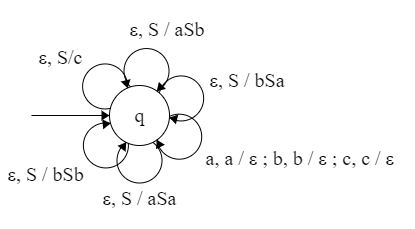
\includegraphics{01.png}
\end{center}

\textbf{в)} Заметим, что это слово не принадлежит языку L, т.к. $|a| \neq |ab|$, работа же построенного МА автомата продеморстрирована на картинке выше.


\subsection{Задача 4}
Coming soon
\subsection{Задача 5}
Coming soon
\subsection{Задача 6}
Язык L задан КС-грамматикой с правилами:
\newline
$S \longrightarrow aSa|aSB|bSa|bSb|a$
\begin{enumerate}
    \item Является ли L регулярным языком?
    \item Является ли дополнение L регулярным языком?
    \item Является ли L КС-языком?
    \item Является ли дополнение L КС-языком?
\end{enumerate}
Изменим немного грамматику из 3-й задачи и получим: $S \longrightarrow aSa|aSb|bSa|bSb|a$
\begin{enumerate}
    \item $L \notin REG$, потому что у него бесконечно много классов L-эквивалентности, к примеру слова, вида b$b^*a$
    \item Сл-но $\Sigma^* \ L \notin REG$
    \item Да, по причине того, что он задается КС-грамматикой
    \item Распишем $T^* \ L = L_1 \cup L_2$
    $L_1 = \{ \omega : \omega = ybz, y, z \in \{a, b\}^*, b \in T, |y| = |z| \}\}$, 
    $L_2 = \{ \omega : |\omega| = 2n, n \geqslant 0\}$
\end{enumerate}
Язык $L_1$ будет задаваться такой же грамматикой, что и L, только нужно заменить $S \longrightarrow a$ на правило $S \longrightarrow b$. Сл-но язык $L_2 \in CFL$ 
\newline
Язык $L_2$ будет задаваться такой же грамматикой, что и L, только нужно заменить правило $S \longrightarrow a$ на $S \longrightarrow \varepsilon$. Сл-но язык $L_2 \in CFL$.
Т.к. КС-языки замкнуты относительно операции объединения, получаем, что $T^* \ L \in CFL$
\subsection{Задача 7}
Язык L задан КС-грамматикой с правилами:
\newline
$S \longrightarrow aSb|A|B|\varepsilon$, $A \longrightarrow aAa|\varepsilon, B \longrightarrow bBb|\varepsilon$
\begin{enumerate}
    \item Является ли L регулярным языком?
    \item Является ли дополнение L регулярным языком?
    \item Является ли L КС-языком?
    \item Является ли дополнение L КС-языком?
\end{enumerate}

\textbf{1.} После k правил $S \longrightarrow aSb$, получим:
\begin{enumerate}
    \item $S \longrightarrow A$, получим слово $\omega = a^{n+2k}b^n$
    \item $S \longrightarrow B$, получим слово $\omega = a^nb^{n+2k}$
    \item $S \longleftarrow \varepsilon$, получим слово $\omega = a^nb^n$
\end{enumerate}
Если n - четна, то есть два случая:
\newline
\textbf{1. } $\omega = a^{2(m+k)}b^{2m}$
\newline
\textbf{2. } $\omega = a^{2m}b^{2(m+k)}$
\newline
Если n - нечетна, то есть два случая;
\newline
\textbf{3.} $\omega = a^{2(m+k)}abb^{2m}$
\newline
\textbf{4.} $\omega = a^{2k}abb^{2(m+k)}$
\newline
Составим регуляргое выражение, которое будет задавать язык L:
\newline
$R = (aa)^*ab(bb)^*|(aa)^*(bb)^*$

\begin{enumerate}
    \item Т.к. есть регулярное выражние, то язык будет регулярным.
    \item Также дополнение язык будет регулярным, это следует из того, что дополнение регулярного языка регулярно.
    \item Он будет КС-языком, т.к. он задаётся грамматикой.
    \item Да, т.к. дополнение языка является регулярным языком, следовательно и КС-языком.
\end{enumerate}




\end{document}